\chapter{Formato BVH}

El formato \emph{BVH} fue originalmente desarrollado por \emph{Biovision}, una empresa especializada en captura de movimiento, como una forma de entregar los datos a sus clientes. El formato consta de dos grandes partes: \emph{HIERARCHY} y \emph{MOTION}. El sistema de captura de movimiento reduce la grabación a un cuerpo rígido, la primera parte describe la jerarquía de ese cuerpo rígido, es decir, como se conectan los segmentos. La segunda parte describe el movimiento. A continuación se describe cada una de las partes.

\section{HIERARCHY}

La jerarquía del cuerpo rígido se expresa como un árbol, cada articulación se asocia a un nodo y se tiene un nodo raíz (comúnmente la cadera). Los segmentos rígidos del cuerpo son entonces los vectores entre dos nodos, donde uno es el padre del otro. El formato especifica utilizar llaves (\mono{\{\}}) para establecer la jerarquía. 

La figura \ref{fig:palitos} muestra un cuerpo rígido humanoide simplificado, según el formato existen tres tipos de nodos: \mono{ROOT} el cual indica que ese es el nodo raíz, \mono{JOINT} indica un nodo (articulación) común, y la palabra \mono{END} indica un nodo terminal. Además de la jerarquía, para cada nodo se establecen dos valores: \emph{OFFSET} y \emph{CHANNELS}. El offset del \mono{ROOT} establece la posición de ese nodo en el marco global, después el offset de cada nodo expresa la posición de ese nodo en el marco local del nodo padre, es decir: considere existe un marco local para cada nodo, donde este es el origen y el offset de los nodos hijos está dado respecto a este origen. 

Los valores channel indican la cantidad de valores necesarios para expresar el movimiento de esa unión. Para el \mono{ROOT} se necesitan al menos 6 canales: 3 para la posición respecto al origen global y 3 para expresar la rotación del vector. Los nodos \mono{JOINT} requieren 3 canales, para expresar su rotación en el marco de referencia del nodo padre. Los nodos \mono{END} no rotan respecto a su padre y no requieren ningún canal. Como consecuencia de los mencionado, note que la distancia entre un nodo hijo y un nodo padre permanece siempre constante, lo que cambia es su rotación y se expresa en el marco de referencia local del padre. 

\begin{minipage}{0.5\textwidth}
\centering
    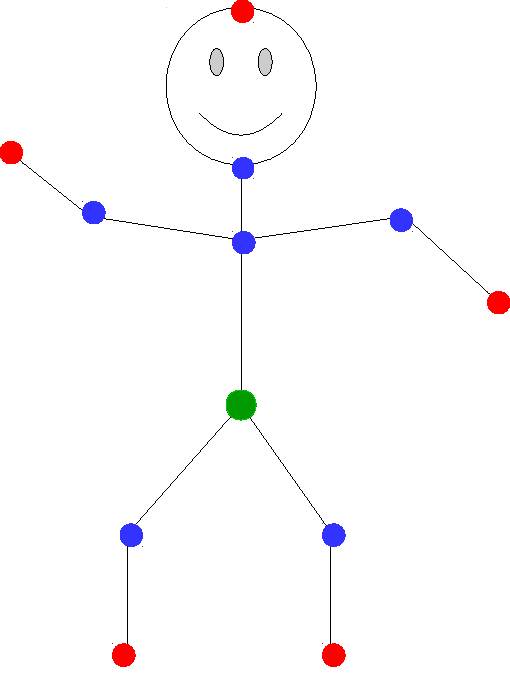
\includegraphics[height = 0.70\textwidth]{imagenes/palitos}
    \captionof{figure}{Cuerpo rígido de ejemplo. Nodo root en verde, nodos en azul y nodos terminales en rojo. A la derecha, ejemplo de como se describe la jerarquía.}
    \label{fig:palitos}
\end{minipage}
\begin{minipage}{0.5\textwidth}
    \begin{verbatim}
ROOT Cadera{
    JOINT PiernaDerecha{
        END PiernaDerecha{
        }
    }
    JOINT PiernaIzquierda{
        END PiernaIzquierda{
        }
    }
    JOINT Pecho{
        JOINT BrazoDerecho{
            END BrazoDerecho{
            }
        }
        JOINT BrazoIzquierdo{
            END Brazo Izquierdo{
            }
        }
        JOINT Cabeza{
            END Cabeza{
            }
        }
    }
}
    \end{verbatim}    
\end{minipage}

La figura \ref{code:joint} muestra la implementación de la estructura \mono{Joint} utilizada para \emph{parsear} la jerarquía de un archivo BVH. Al encontrar la palabra reservada \mono{ROOT}, \mono{JOINT} o \mono{END} se crea un nuevo Joint y se añade a un arreglo, excepto en el caso del ROOT, el puntero padre apunta al último Joint añadido al arreglo de padres. Al encontrar una llave izquierda \mono{\{} se toma el último Joint del arreglo Joints y se añade a un arreglo de padres, al encontrar una llave derecha \mono{\}} se elimina el último Joint del arreglo de padres. 

La siguiente sección explicará en detalle la función de las matices locales y globales, por ahora basta con decir que el valor de offset se almacena en la última columna de la matriz local. 

\begin{figure}
    \centering
    \begin{verbatim}
struct Joint{
    char * name;
    int isRoot;
    int isEnd;
    Joint * parent;
    double rotation[3];
    double * local_matrix;
    double * global_matrix;
}
    \end{verbatim}
    \caption{Implementación de la estructura \mono{Joint}}
    \label{code:joint}
\end{figure}

\section{MOTION}

Esta sección inicia con la palabra reservada \mono{MOTION}, a continuación se encuentran los valores \mono{Frames}, indica la cantidad de frames de la filmación y la palabra \mono{Frame time} que indica el periodo entre frames (el inverso de la frecuencia de grabación). Cada frame consiste en 6 valores en decimal para expresar el movimiento del nodo ROOT (3 para actualizar su posición global y 3 para su rotación) y 3 valores por cada Joint que no sea End. 

La matriz global y local de cada joint es una matriz $4 \times 4$, conformado por cuatro vectores columna, los primeros tres expresan rotación y siguiendo la convención en computación de graficos, tiene un cero en la cuarta fila. El cuarto vector columna expresa traslación y siguiendo la convención, tiene un uno en la cuarta fila, la ecuación \eqref{matriz_general} muestra esta convención.

\begin{equation}\label{matriz_general}
M = 
    \begin{pmatrix}
    r_{xx} & r_{xy} & r_{xz} & t_x \\
    r_{yx} & r_{yy} & r_{yz} & t_y \\
    r_{zx} & r_{zy} & r_{zz} & t_z \\
    0      & 0      & 0      & 1 
    \end{pmatrix}
\end{equation}

Los valores $t$ corresponden al offset encontrado en la sección \mono{HIERARCHY}, los valores $r$ Se obtiene la multiplicar las matrices de rotación $R_z$, $R_y$ y $R_x$, como se muestra en \eqref{matriz_rotacion}, los valores de los ángulos representados por $\theta$ en la ecuación son los valores que aparecen en esta sección, como se puede observar, son tres por Joint para formar la matriz. 

\begin{equation}\label{matriz_rotacion}
R_z R_y R_x = 
\begin{pmatrix}
 cos\ \theta_z & - sin\ \theta_z & 0 \\
 sin\ \theta_z & cos\ \theta_z & 0 \\
 0 & 0 & 1 
\end{pmatrix}
\begin{pmatrix}
 cos\ \theta_y & 0 & sin\ \theta_y \\
 0 & 1 & 0 \\
 - sin\ \theta_y & 0 & cos\ \theta_y 
\end{pmatrix}
\begin{pmatrix}
 1 & 0 & 0 \\
 0 & cos\ \theta_x & - sin\ \theta_x \\
 0 & sin\ \theta_x & cos\ \theta_x 
\end{pmatrix}
\end{equation}

En el caso de ROOT, la matriz global y local son la misma, pues el nodo ROOT existe en el marco de referencia global, para los demás nodos, se construye la matriz local, tal como se explicó anteriormente y se multiplica por la matriz global del nodo padre, claramente esta es una acción recursiva, pues se debe llegar hasta el nodo ROOT, como se muestra a continuación \eqref{matriz_recursiva}.

\begin{equation}\label{matriz_recursiva}
    M_{\text{global}} = M_{\text{local}} M_{\text{global\_padre}} M_{\text{global\_abuelo}} ... M_{\text{global\_root}}
\end{equation}

Finalmente, la posición de cada nodo respecto al marco de referencia global se encuentra en el cuarto vector columna de la matriz global. 
    El siguiente es un extracto de un archivo BVH con su primer frame.

\begin{verbatim}
HIERARCHY
ROOT Hips
{
  OFFSET 0.000000 0.000000 0.000000
  CHANNELS 6 Xposition Yposition Zposition Zrotation Xrotation Yrotation
  JOINT Spine
  {
    OFFSET -0.000000 0.076886 0.000000
    CHANNELS 3 Zrotation Xrotation Yrotation
    JOINT Spine1
    {
      OFFSET -0.000000 0.200136 0.000000
      CHANNELS 3 Zrotation Xrotation Yrotation
      JOINT Neck
      {
        OFFSET -0.000000 0.199314 0.018119
        CHANNELS 3 Zrotation Xrotation Yrotation
        JOINT Head
        {
          OFFSET -0.000000 0.131269 -0.018753
          CHANNELS 3 Zrotation Xrotation Yrotation
          End Site
          {
            OFFSET -0.000000 0.187528 0.000000
          }
        }
      }
      JOINT LeftShoulder
      {
        OFFSET 0.037527 0.175039 -0.003779
        CHANNELS 3 Zrotation Xrotation Yrotation
        JOINT LeftArm
        {
          OFFSET 0.133636 0.000000 0.000000
          CHANNELS 3 Zrotation Xrotation Yrotation
          JOINT LeftForeArm
          {
            OFFSET 0.299034 0.000000 0.000000
            CHANNELS 3 Zrotation Xrotation Yrotation
            JOINT LeftHand
            {
              OFFSET 0.221443 0.000000 0.000000
              CHANNELS 3 Zrotation Xrotation Yrotation
              End Site
              {
                OFFSET 0.140646 0.000000 0.000000
              }
            }
          }
        }
      }
      JOINT RightShoulder
      {
        OFFSET -0.037320 0.175039 -0.003779
        CHANNELS 3 Zrotation Xrotation Yrotation
        JOINT RightArm
        {
          OFFSET -0.133636 0.000000 0.000000
          CHANNELS 3 Zrotation Xrotation Yrotation
          JOINT RightForeArm
          {
            OFFSET -0.299034 0.000000 0.000000
            CHANNELS 3 Zrotation Xrotation Yrotation
            JOINT RightHand
            {
              OFFSET -0.221443 0.000000 0.000000
              CHANNELS 3 Zrotation Xrotation Yrotation
              End Site
              {
                OFFSET -0.140646 0.000000 0.000000
              }
            }
          }
        }
      }
    }
  }
  JOINT LeftUpLeg
  {
    OFFSET 0.093764 0.000000 0.000000
    CHANNELS 3 Zrotation Xrotation Yrotation
    JOINT LeftLeg
    {
      OFFSET -0.000000 -0.396379 0.000000
      CHANNELS 3 Zrotation Xrotation Yrotation
      JOINT LeftFoot
      {
        OFFSET -0.000000 -0.402188 0.000000
        CHANNELS 3 Zrotation Xrotation Yrotation
        JOINT LeftToeBase
        {
          OFFSET -0.000000 -0.060946 0.140646
          CHANNELS 3 Zrotation Xrotation Yrotation
          End Site
          {
            OFFSET -0.000000 0.000000 0.037506
          }
        }
      }
    }
  }
  JOINT RightUpLeg
  {
    OFFSET -0.093764 0.000000 0.000000
    CHANNELS 3 Zrotation Xrotation Yrotation
    JOINT RightLeg
    {
      OFFSET -0.000000 -0.396379 0.000000
      CHANNELS 3 Zrotation Xrotation Yrotation
      JOINT RightFoot
      {
        OFFSET -0.000000 -0.402188 0.000000
        CHANNELS 3 Zrotation Xrotation Yrotation
        JOINT RightToeBase
        {
          OFFSET -0.000000 -0.060946 0.140646
          CHANNELS 3 Zrotation Xrotation Yrotation
          End Site
          {
            OFFSET -0.000000 0.000000 0.037506
          }
        }
      }
    }
  }
}
MOTION
Frames:    19765
Frame Time:    0.003906
3.559094    0.923209    0.525318    0.013638    0.239340    -92.314423    -0.866819    
-8.201900   -1.085093    0.390321    1.095642    -0.341925    11.942478    19.273811
6.916184    -14.095366    1.028759    5.660420    16.413609    3.670976    6.878858
-20.665810  -4.967050    -7.953991    -9.244185    7.996674    -9.049491    -0.397082
7.268273    0.493494    -11.031128    2.884695    3.247415    18.525766    3.898051
3.358436    10.172389    6.814506    11.962240    1.635878    5.769930    1.235742
1.274122    6.534966    4.544692    -3.154521    -1.556152    -2.001814    1.299514
-4.085289    6.960749    0.023962    0.327613    -0.119950    -1.233113    4.604572
-3.182750    2.910497    5.662087    0.776524    -0.874389    -9.110942    -3.389380
-0.066035    -0.925920    0.191887    
\end{verbatim}

\chapter{Algoritmo de detección de los pasos}
